\documentclass{article}
\usepackage[utf8]{inputenc}
\usepackage{CJKutf8}
\usepackage{amsmath}
\usepackage{algorithm}
\usepackage[noend]{algpseudocode}

\makeatletter
\def\BState{\State\hskip-\ALG@thistlm}
\makeatother

\title{Computer Architecture: Project \#2}

\begin{CJK}{UTF8}{bsmi}

\author{b07902047 羅啟帆\\ b07902139 鄭豫澤}
\date{December 2019}

\usepackage{natbib}
\usepackage{amsmath}
\usepackage{indentfirst}
\usepackage{hyperref}
\usepackage{amssymb}
\usepackage{graphicx}
\usepackage[a4paper, total={6.5in, 10in}]{geometry}

\usepackage{listings}
\usepackage{color}

\definecolor{codegreen}{rgb}{0,0.6,0}
\definecolor{codegray}{rgb}{0.5,0.5,0.5}
\definecolor{codepurple}{rgb}{0.58,0,0.82}
\definecolor{backcolour}{rgb}{0.95,0.95,0.92}

\lstdefinestyle{mystyle}{
    backgroundcolor=\color{backcolour},
    commentstyle=\color{codegreen},
    keywordstyle=\color{magenta},
    numberstyle=\tiny\color{codegray},
    stringstyle=\color{codepurple},
    basicstyle=\footnotesize,
    breakatwhitespace=false,
    basicstyle=\ttfamily,
    columns=fullflexible,
    frame=single,
    breaklines=true,
    captionpos=b,
    keepspaces=true,
    numbers=left,
    numbersep=5pt,
    showspaces=false,
    showstringspaces=false,
    showtabs=false,
    tabsize=4
}

\lstset{style=mystyle}


\begin{document}

\maketitle

%\setcounter{secnumdepth}{0}

\section{Implementation}

We connected new modules in CPU first, then starting working on cache. We encountered lots of strange bug during the implementation, therefore we printed lots of things(the commented block in testbench). Note that our implementation of "read value" of the line that is "read miss" will print the value that will be written back to data memory.

\section{Cache Controller}

\begin{center}
    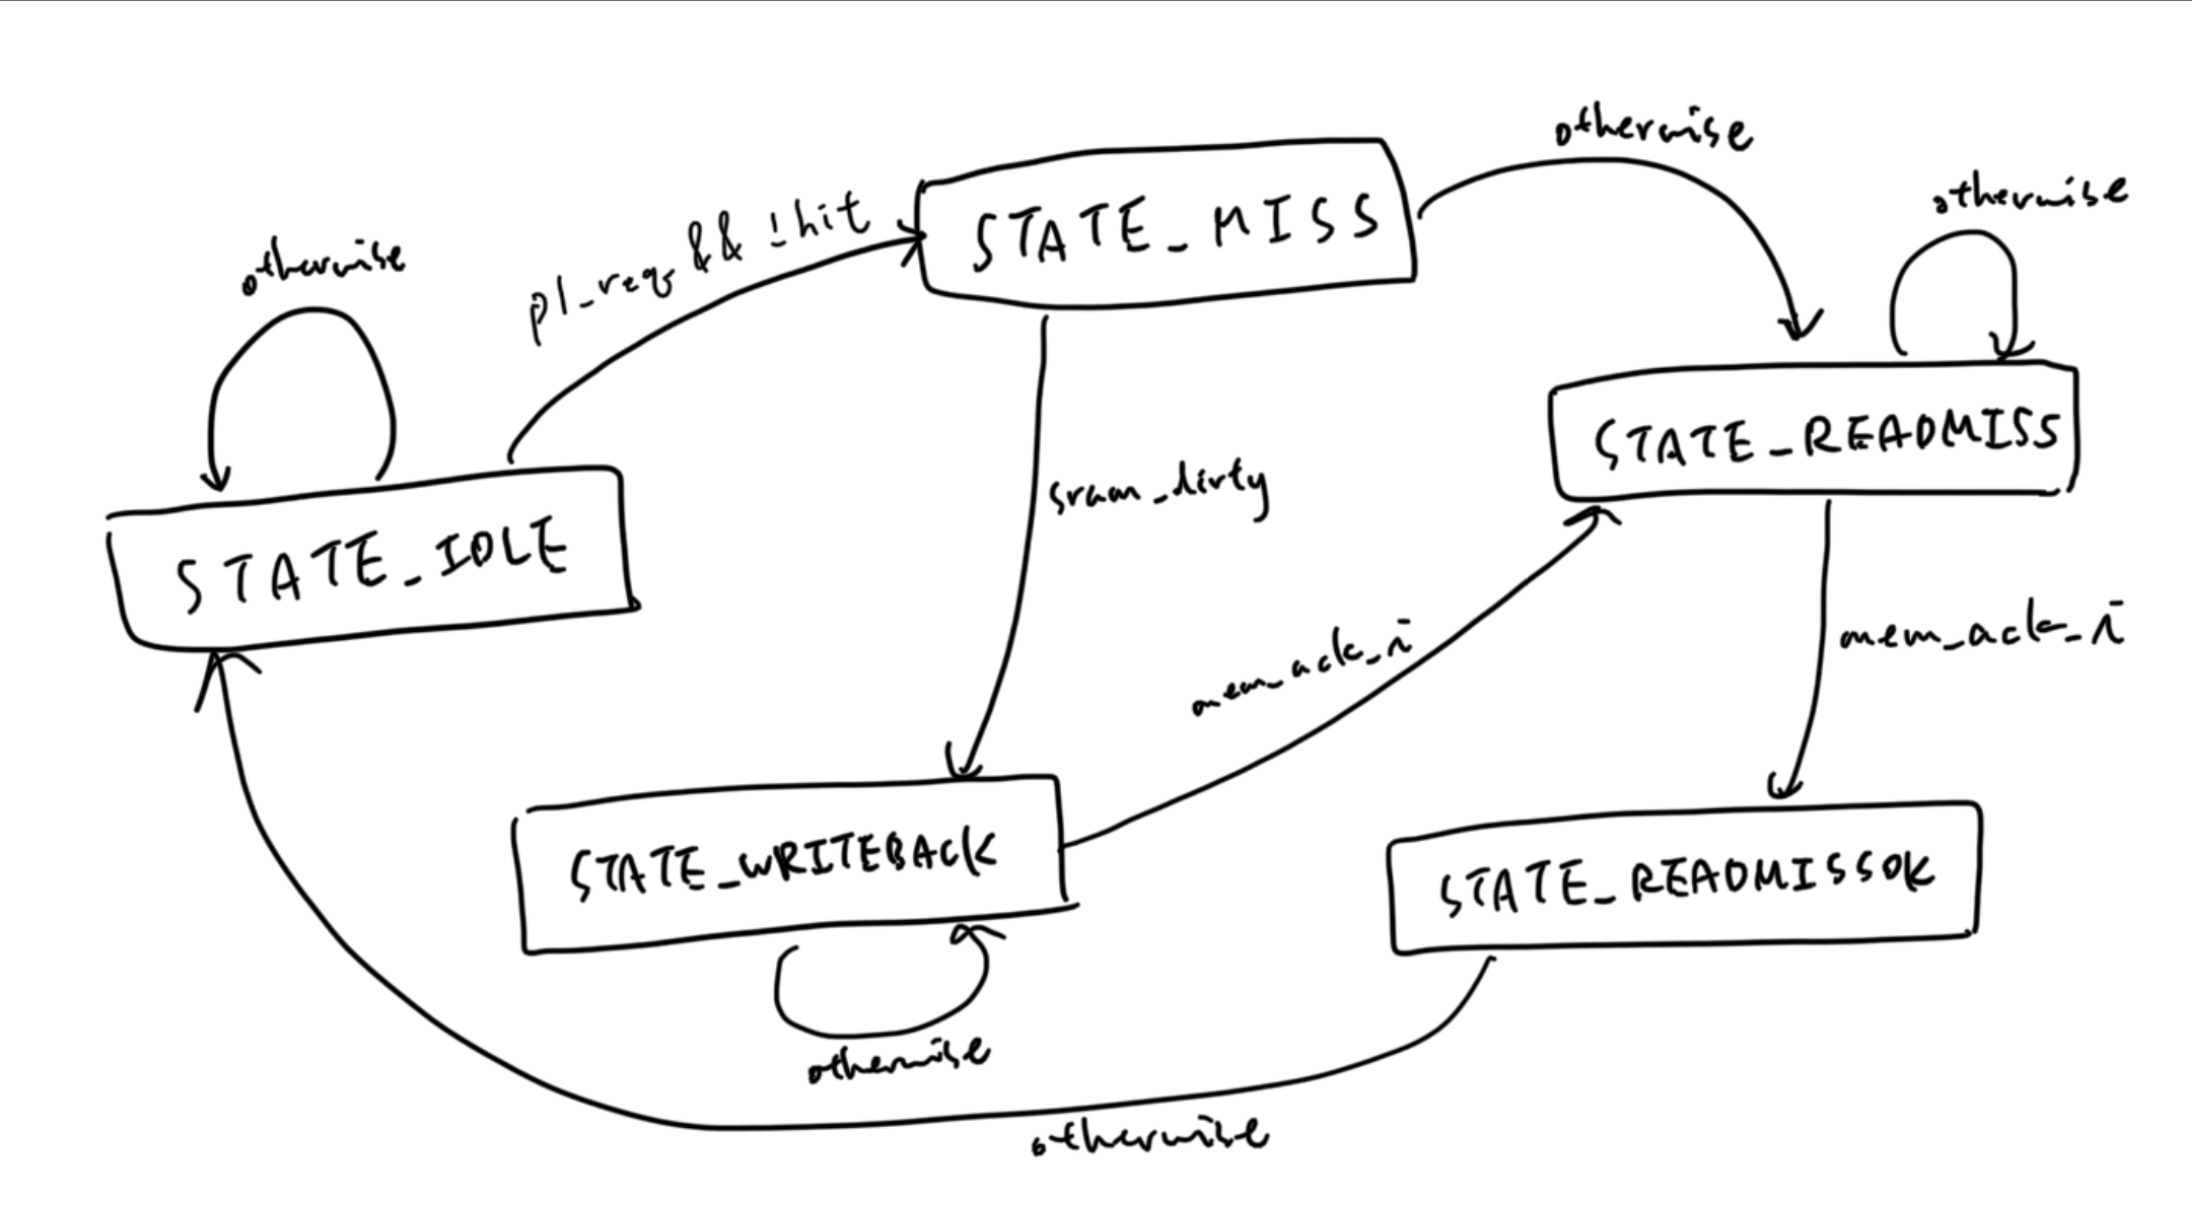
\includegraphics[scale=0.25]{pp}
\end{center}

The condition to transfer between states is given on the edges. When we transfer from one edge to another, we also modify four variables(\textit{mem\_enable, mem\_write, cache\_we, write\_back}) to appropriate values.

\section{Difficulties}

Didn't notice that Q\&A section under the homework website has been updated(no email is sent or something), and debugged for several hours...Also, it take time to understand the given code, maybe more comments will help a lot.

\section{Work division}

We do this project together
\begin{enumerate}
    \item Code: b07902047 \& b07902139
    \item Report: b07902047 \& b07902139
\end{enumerate}

\end{document}

\end{CJK}
